\usetikzlibrary{matrix,backgrounds,positioning,calc,fit}
\definecolor{commentColor}{RGB}{102,102,102}
\definecolor{commandColor}{RGB}{59,61,196}

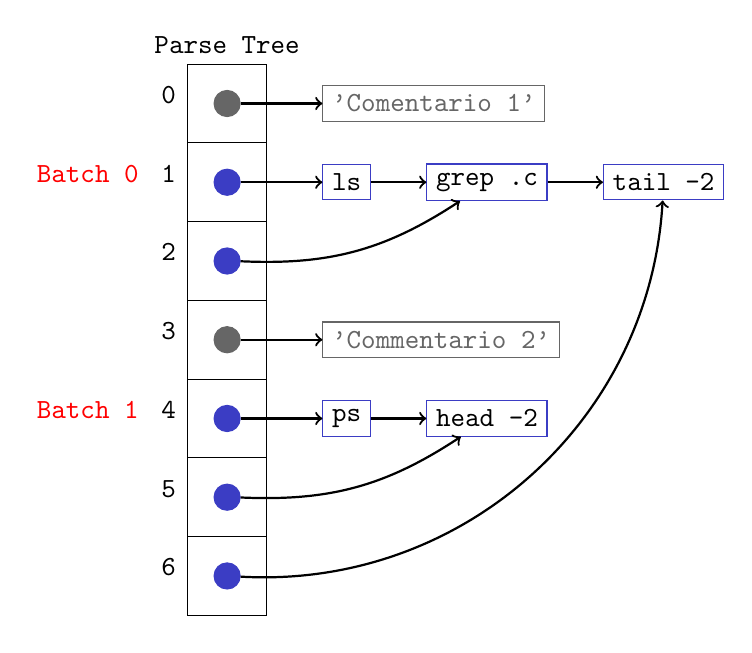
\begin{tikzpicture}[font=\ttfamily,
varray/.style={
    matrix of nodes,nodes={
        draw, minimum size=10mm, fill=white!30},
    column sep=-\pgflinewidth,
    row sep=-\pgflinewidth,
    nodes in empty cells,
    column 1/.style={
        nodes={
            draw=none, fill=none, minimum size=5mm
        }
    }
},
harray/.style={
    matrix of nodes, nodes={
        draw, minimum size=2mm, fill=white!30},
    column sep=-\pgflinewidth,
    row sep=-\pgflinewidth,
    nodes in empty cells,
    row 1/.style={
        nodes={
            draw=none, fill=none, minimum size=5mm
        }
    }
},
cmdPtr/.style={
    draw, commandColor, fill=commandColor, minimum size=2mm, circle
},
cmtPtr/.style={
    draw, commentColor, fill=commentColor, minimum size=2mm, circle
}]

\newdimen\zerolinewidth

\tikzset{
    zero line width/.code={
        \zerolinewidth=\pgflinewidth
        \tikzset{line width=0cm}
    },
    use line width/.code={
        \tikzset{line width=\the\zerolinewidth}
    },
    anchor-in-boundary/.style={
        zero line width,
        postaction={draw,use line width},
    },
}

\matrix[varray] (parseTree) {
0 &    \\
1 &    \\
2 &    \\
3 &    \\
4 &    \\
5 &    \\
6 &    \\
};
\draw (parseTree-1-2.north)++ (60:0mm) node [above] (ptLabel) {Parse Tree};

% Comment 1
    \node[cmtPtr] at (parseTree-1-2) (cmt1ptr) {};
    \node[draw, commentColor, right = 20pt of parseTree-1-2.east]
        (cmt1) {'Comentario 1'};
    \draw[->, thick] (cmt1ptr)--(cmt1);

% Command 1 LS
    \node[cmdPtr] at (parseTree-2-2) (cmdLSPtr) {};
    \node[draw, commandColor, text=black, right = 20pt of parseTree-2-2.east]
        (cmdLS) {ls};
    \draw (parseTree-2-1.west)++(0:0mm) node [left, text=red]
        (batch0Label) {Batch 0};

% Command 2 Grep
    \node[cmdPtr] at (parseTree-3-2) (cmdGrepPtr) {};
    \node[draw, commandColor, text=black, right = 20pt of cmdLS.east]
        (cmdGrep) {grep .c};

% Comment 1
    \node[cmtPtr] at (parseTree-4-2) (cmt2ptr) {};
    \node[draw, commentColor, right = 20pt of parseTree-4-2.east]
        (cmt2) {'Commentario 2'};
    \draw[->, thick] (cmt2ptr)--(cmt2);

% Command 3 PS
    \node[cmdPtr] at (parseTree-5-2) (cmdPSPtr) {};
    \node[draw, commandColor, text=black, right = 20pt of parseTree-5-2.east]
        (cmdPS) {ps};
    \draw (parseTree-5-1.west)++(0:0mm) node [left, text=red]
        (batch1Label) {Batch 1};

% Command 4 Head
    \node[cmdPtr] at (parseTree-6-2) (cmdHeadPtr) {};
    \node[draw, commandColor, text=black, right = 20pt of cmdPS.east]
        (cmdHead) {head -2};

% Command 5 Tail
    \node[cmdPtr] at (parseTree-7-2) (cmdTailPtr) {};
    \node[draw, commandColor, text=black, right = 20pt of cmdGrep.east]
        (cmdTail) {tail -2};

\foreach \from/\to in {cmdLSPtr/cmdLS, cmdLS/cmdGrep, cmdGrep/cmdTail,
                        cmdPSPtr/cmdPS, cmdPS/cmdHead}
    \draw [->, thick] (\from)--(\to);

\draw[->, thick, bend right=18] (cmdGrepPtr) edge (cmdGrep);

\draw[->, thick, bend right=18] (cmdHeadPtr) edge (cmdHead);

\draw[->, thick, bend right=45] (cmdTailPtr) edge (cmdTail);

\end{tikzpicture}
